\documentclass[twosided]{report}

% Packages %
\usepackage{fancyhdr}
\usepackage{titling}
\usepackage{graphicx}
\usepackage{xcolor}
\usepackage{listings}
\usepackage{algorithm}
\usepackage{algorithmic}
\usepackage{framed}

% Stylings %
\pagestyle{fancy}

% Commands %
\newcommand{\subtitle}[1]{%
  \posttitle{%
    \par\end{center}
    \begin{center}\large#1\end{center}
    \vskip0.5em}%
}

% Colors %
\definecolor{darkgreen}{RGB}{60, 100, 60}
\definecolor{purple}{RGB}{170, 0, 210}
\definecolor{lightyellow}{RGB}{255, 251, 204}
\definecolor{navy}{RGB}{40, 55, 170} 
\definecolor{myblue}{rgb}{0.25, 0.25, 0.645} 
\definecolor{darkred}{rgb}{0.845, 0.125, 0.125} 
\definecolor{grey}{RGB}{100, 100, 100}
\definecolor{sblbackground}{RGB}{39, 40, 34}
\definecolor{sblkeyword}{RGB}{246, 39, 113}
\definecolor{sbltext}{RGB}{248, 242, 242}
\definecolor{sblcomment}{RGB}{94, 109, 94}
\definecolor{sblstring}{RGB}{230, 219, 101}
\definecolor{shadecolor}{named}{sblbackground} 

% Footer/Header %
\fancyhead[LE,RO]{\slshape Chapter \thechapter}
\fancyhead[LO,RE]{\slshape \rightmark}
\fancyfoot[C]{\thepage}

\newcommand{\HRule}{\rule{\linewidth}{0.5mm}}

\lstdefinestyle{fstar}{
	backgroundcolor=\color{sblbackground},
	tabsize=1,
	captionpos=b
  	belowcaptionskip=1\baselineskip,
  	breaklines=true,
  	frame=single,
	%frameround=tttt,
	captionpos=b,
  	language=Caml,
	morekeywords={open, module, val, assert},
	showspaces=false,
  	showstringspaces=false,
	showtabs=false,
  	numbers=left,
  	numbersep=5pt,
  	numberstyle=\tiny\ttfamily\color{grey},
	xleftmargin=\parindent,
  	basicstyle=\footnotesize\ttfamily\color{sbltext},
  	keywordstyle=\bfseries\color{sblkeyword},
	otherkeywords={=, :, |},
  	stringstyle=\color{sblstring},
	commentstyle=\color{sblcomment},
	%literate={0}{\textcolor{blue}{0}}
}

\begin{document}

\begin{titlepage}
\begin{center}


\includegraphics[scale=0.4]{images/ITULogo.jpg}\\[1cm]

\textsc{\LARGE IT University of Copenhagen}\\[1.5cm]

\textsc{\Large Bachelor Project}\\[0.5cm]

% Title
\HRule \\[0.4cm]
{\huge \bfseries Verifiable Secure Open Source Alternative to NemID}\\[0.1cm]
\HRule \\[1.5cm]

% Author and supervisor
\begin{minipage}[t]{0.45\textwidth}
\begin{flushleft} \large
\emph{Authors:}
\\[10pt]
Andreas Hallberg \textsc{Kjeldsen}\\
\emph{ahal@itu.dk}
\\[10pt]
Morten Chabert \textsc{Eskesen}\\
\emph{mche@itu.dk}\\
\end{flushleft}
\end{minipage}
\begin{minipage}[t]{0.45\textwidth}
\begin{flushright} \large
\emph{Supervisor:}
\\[10pt]
Joseph Roland \textsc{KINIRY}\\
\emph{josr@itu.dk}
\end{flushright}
\end{minipage}

\vfill

% Bottom of the page
{\large May 22, 2013}

\end{center}
\end{titlepage}


\begin{abstract}
Your abstract goes here...
\end{abstract}

\tableofcontents

\chapter{Introduction}

$\ldots$
\par
We're extending the work done by Jacob Højgaard in his Masters Thesis 'Securing Single Sign-On Systems With Executable Models'. Jacobs research has focused on the current implementation of NemID and therefore describes, outlines and models the current system used in Denmark as of May 2013.

\section{Objectives}
Some explaining text here
\par

\begin{enumerate}
	\item Describe and outline the OpenNemID protocol, including but not limited to registration and login.
	\item Formalize the specification of OpenNemID in F* to the extent possible.
\end{enumerate}

\section{Scope}
This project has had it focus towards specifying a new protocol that could replace NemID. The intent of this project is therefore not to develop a complete system, but to make the specification for a system that could then later be developed based on the specification.

\section{Background}
$\ldots$
 
\chapter{Technical Background}

\section{SAML Protocol}

\section{Static Analysis}

\section{Selection of verification tool}

\section{N Factor Authentication}
Videreudvikling af two factor authentication


%%%%%%%%%% CHAPTER %%%%%%%%%%
\chapter{Remodelling the protocol}
\section{How It Is Today}

\section{How It Could Be}

\section{Communication Model}
The communication model displays a graphical overview of how data should be communicated between the involved parties.
\newpage
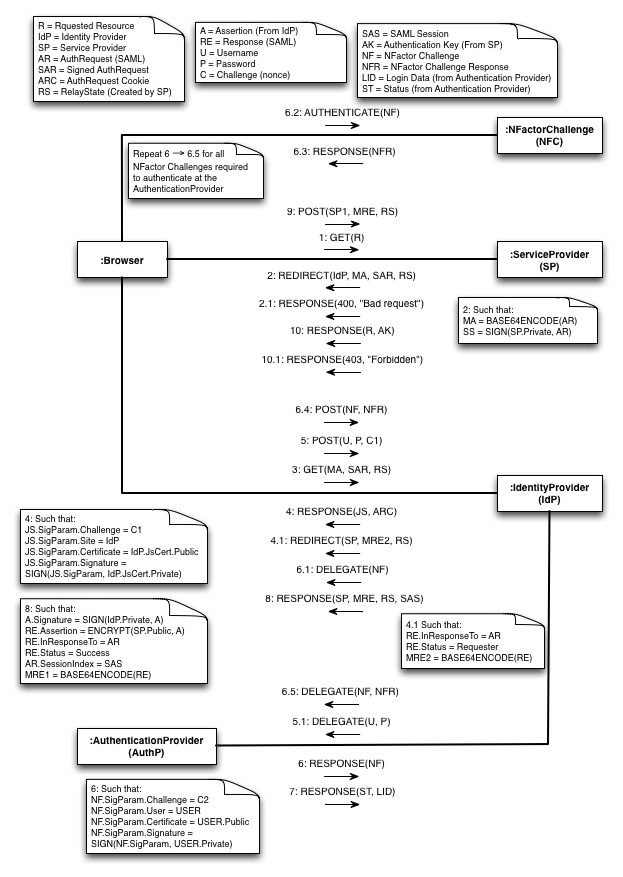
\includegraphics[scale=0.6]{images/Communication.png}

TEXT DESCRIBING ALGORITHM 1
\begin{algorithm}[H]
	\caption{Process 1}
	\begin{algorithmic}
	\REQUIRE{GET is well-formed \AND IdP.Public \AND SP.Private}
	\IF{R exists}
		\STATE AR $\leftarrow$ CreateAuthnRequest()
		\STATE SAR $\leftarrow$ SIGN(AR, SP.Private)
		\STATE MA $\leftarrow$ UrlEnc(Base64Enc(DeflateCompress(AR)))
		\STATE RS $\leftarrow$ UrlEnc(Base64Enc(R))
		\RETURN REDIRECT(IdP, MA, SAR, RS)
	\ELSE
		\RETURN RESPONSE(400, Bad−Request)
	\ENDIF
	\end{algorithmic}
\end{algorithm}

TEXT DESCRIBING ALGORITHM 2
\begin{algorithm}[H]
	\caption{Process 3}
	\begin{algorithmic}
		\REQUIRE{GET is well-formed \AND IdP.Private \AND SP.Public \AND IdPJsCert.Public \AND IdP has JavaScript from AuthP}
		\STATE AR $\leftarrow$ DeflateDecompress(Base64Dec(UrlDec(MA)))
		\IF{VERIFY(AR, SAR, SP.Public)}
			\STATE C1 $\leftarrow$ GenChallenge()
			\STATE JS $\leftarrow$ StoredJavaScript()
			\STATE JS.SigParams.Challenge $\leftarrow$ C1
			\STATE JS.SigParams.Certificate $\leftarrow$ IdPJsCert.Public
			\STATE JS.SigParams.Signature $\leftarrow$ SIGN(JS.SigParams, IdPJsCert.Private)
			\RETURN RESPONSE(JS)
		\ELSE
			\STATE RE $\leftarrow$ CreateResponse()
			\STATE RE.InResponseTo $\leftarrow$ AR
			\STATE RE.Status $\leftarrow$ ”Requester”
			\STATE MRE $\leftarrow$ Base64Enc(RE)
			\RETURN REDIRECT(SP, MRE, RS)
		\ENDIF
	\end{algorithmic}
\end{algorithm}

TEXT DESCRIBING ALGORITHM 3
\begin{algorithm}[H]
	\caption{Process 4}
	\begin{algorithmic}
		\REQUIRE{U \AND P \AND Browser allows JavaScript}
		\STATE SigParams $\leftarrow$ Js.SigParams
		\IF{VERIFY(SigParams, SigParams.Signature, SigParams.Certificate)}
			\STATE C1 $\leftarrow$ SigParams.Challenge
			\RETURN POST(U, P, C1)
		\ELSE
			\PRINT ERROR
		\ENDIF
	\end{algorithmic}
\end{algorithm}

TEXT DESCRIBING ALGORITHM 4
\begin{algorithm}[H]
	\caption{Process 5}
	\begin{algorithmic}
		\REQUIRE{POST is well formed}
		\IF{C1 matches challenge issued by IdP}
			\STATE \textbf{Delegate} U \AND P \TO AuthP
		\ELSE
			\RETURN RESPONSE(ERROR)
		\ENDIF
		\REQUIRE{C1 matches challenge issued by IdP}
	\end{algorithmic}
\end{algorithm}

TEXT DESCRIBING ALGORITHM 5
\begin{algorithm}[H]
	\caption{Process 5.1}
	\begin{algorithmic}
		\STATE USER $\leftarrow$ GetUser(U, P)
		\IF{USER is valid}
			\STATE C2 $\leftarrow$ GenChallenge()
			\STATE NF $\leftarrow$ GetNextNFactorChallenge(USER)
			\STATE NF.SigParam.User $\leftarrow$ USER
			\STATE NF.SigParam.Challenge $\leftarrow$ C2
			\STATE NF.SigParam.Certificate $\leftarrow$ USER.Public
			\STATE NF.SigParam.Signature $\leftarrow$ SIGN(NF.SigParam, USER.Private)
			\RETURN RESPONSE(NF)
		\ELSE
			\RETURN RESPONSE(ERROR)
		\ENDIF
	\end{algorithmic}
\end{algorithm}

TEXT DESCRIBING ALGORITHM 6
\begin{algorithm}[H]
	\caption{Process 6}
	\begin{algorithmic}
		\STATE SigParams $\leftarrow$ NF.SigParams
		\IF{VERIFY(SigParams, SigParams.Signature, SigParams.Certificate)}
			\STATE RELATE(SigParams.User, SigParams.Challenge)
			\STATE \textbf{Delegate} NF \TO Browser
		\ELSE
			\STATE \textbf{Delegate} ERROR \TO Browser
		\ENDIF
	\end{algorithmic}
\end{algorithm}

TEXT DESCRIBING ALGORITHM 7
\begin{algorithm}[H]
	\caption{Process 6.1}
	\begin{algorithmic}
		\STATE SigParams $\leftarrow$ NF.SigParams
		\IF{VERIFY(SigParams, SigParams.Signature, SigParams.Certificate)}
			\STATE AUTHENTICATE(NF)
		\ELSE
			\PRINT ERROR
		\ENDIF
	\end{algorithmic}
\end{algorithm}

TEXT DESCRIBING ALGORITHM 8
\begin{algorithm}[H]
	\caption{Process 6.2}
	\begin{algorithmic}
		\STATE NFR $\leftarrow$ NFactorResult(NF)
		\RETURN RESPONSE(NFR)
	\end{algorithmic}
\end{algorithm}

TEXT DESCRIBING ALGORITHM 9
\begin{algorithm}[H]
	\caption{Process 6.5}
	\begin{algorithmic}
		\REQUIRE{Stored relation for (NF.SigParams.USER, NF.SigParams.Certificate)}
		\STATE SigParams $\leftarrow$ NF.SigParams
		\IF{VERIFY(SigParams, SigParams.Signature, SigParams.Certificate)}
			\IF{NFR is acceptable result of NF}
				\STATE USER $\leftarrow$ GetUser(SigParams.USER, SigParams.Certificate)
				\STATE C2 $\leftarrow$ GenChallenge()
				\IF{USER.HasNextChallenge}
					\STATE NF $\leftarrow$ GetNextNFactorChallenge(USER)
					\STATE NF.SigParams.User $\leftarrow$ USER
					\STATE NF.SigParams.Challenge $\leftarrow$ C2
					\STATE NF.SigParams.Certificate $\leftarrow$ USER.Public
					\STATE NF.SigParams.Signature $\leftarrow$ SIGN(NF.SigParams, USER.Private)
					\RETURN RESPONSE(NF)
				\ELSE
					\STATE LID $\leftarrow$ CreateLogInData()
					\STATE ST $\leftarrow$ ”OK”
					\RETURN RESPONSE(ST, LID)
				\ENDIF
			\ELSE
				\RETURN RESPONSE(ERROR)
			\ENDIF
		\ELSE
			\RETURN RESPONSE(ERROR)
		\ENDIF	
	\end{algorithmic}
\end{algorithm}

TEXT DESCRIBING ALGORITHM 10
\begin{algorithm}[H]
	\caption{Process 7}
	\begin{algorithmic}
		\REQUIRE{SP.Public \AND LID is well-formed \AND stored AuthRequest for (LID.User, LID.Challenge)}
		\IF{ST = "OK"}
			\STATE ARC $\leftarrow$ GetAuthRequest(LID.User, LID.Challenge)
			\STATE MA $\leftarrow$ ARC.AR
			\STATE SAR $\leftarrow$ ARC.SAR
			\STATE RS $\leftarrow$ ARC.RS
			\STATE AR $\leftarrow$ DeflateDecompress(Base64Dec(UrlDec(MA)))
			\IF{VERIFY(AR, SAR, SP.Public)}
				\STATE A $\leftarrow$ BuildAssertion(LID.Certificate)
				\STATE SI $\leftarrow$ GenerateSessionIndex()
				\STATE A.InResponseTo $\leftarrow$ AR
				\STATE A.Issuer $\leftarrow$ IdP
				\STATE A.Audience $\leftarrow$ SP
				\STATE A.SessionIndex $\leftarrow$ SI
				\STATE A.Signature $\leftarrow$ SIGN(A, IdP.Private)
				\STATE EA $\leftarrow$ ENCRYPT(A, SP.Public)
				\STATE RE $\leftarrow$ CreateResponse()
				\STATE RE.Assertion $\leftarrow$ EA
				\STATE RE.InResponseTo $\leftarrow$ AR
				\STATE RE.Status $\leftarrow$ "Success"
				\STATE MRE $\leftarrow$ DeflateCompress(Base64Enc(UrlEnc(RE)))
				\STATE SAS $\leftarrow$ CreateSAMLSession(SI, SP, LID.CertificateSubject)
				\RETURN REDIRECT(SP, MRE, RS, SAS)
			\ELSE
				\STATE RE $\leftarrow$ CreateResponse()
				\STATE RE.InResponseTo $\leftarrow$ AR
				\STATE RE.Status $\leftarrow$ "Requester"
				\STATE MRE $\leftarrow$ DeflateCompress(Base64Enc(UrlEnc(RE)))
				\RETURN REDIRECT(SP, MRE, RS)
			\ENDIF	
		\ELSE
			\RETURN RESPONSE(ST)
		\ENDIF
	\end{algorithmic}
\end{algorithm}

TEXT DESCRIBING ALGORITHM 11
\begin{algorithm}[H]
	\caption{Process 9}
	\begin{algorithmic}
		\REQUIRE{POST is well.formed \AND SP.Private \AND IdP.Public}
		\STATE RE $\leftarrow$ UrlDec(Base64Dec(DeflateDecompress(MRE)))
		\STATE A $\leftarrow$ DECRYPT(RE.Assertion, SP.Private)
		\IF{VERIFY(A, A.Signature, IdP.Public)}
			\STATE AK $\leftarrow$ GenAuthKey()
			\STATE R $\leftarrow$ Base64Dec(UrlDec(RS))
			\STATE RES $\leftarrow$ GetResource(R)
			\RETURN RESPONSE(RES, AK)
		\ELSE
			\RETURN RESPONSE(403, Forbidden)
		\ENDIF
	\end{algorithmic}
\end{algorithm}

\chapter{Modelling with F*}

\section{Introducing F*}

\section{Syntax and semantics}

\section{Refinement types}

\section{Protocol specification in F*}
hello world
\subsection{Specification of the type functionality module}
%\begin{shaded}
\begin{lstlisting}[style=fstar, caption={TypeFunc module}]
	module TypeFunc

	type Authentication =
 	 | Facebook: id:int -> Authentication
 	 | SMS: generated:int -> Authentication
	 | Google: id:int -> Authentication
	 | OpenId: id:int -> Authentication
\end{lstlisting}
%\end{shaded}

\subsection{Specification of the SAML Protocol}
%\begin{shaded}
\begin{lstlisting}[style=fstar, caption={SAML Protocol module}]
	module SamlProtocol
	
	open Crypto
	open TypeFunc

	type assertiontoken = string (*Add refinements*)
	type signedtoken = string (*Add refinements*)
	type id = string
	type endpoint = string
	type uri = string


	type AuthnRequest = 
	  | MkAuthnRequest: IssueInstant:string ->
			    Destination:endpoint -> Issuer:prin ->
			    message:string -> sig:dsig ->
			    AuthnRequest

	type LoginData = 
	  | MkLoginData:  user:prin -> signature:dsig ->
			  cert:pubkey user -> challenge:nonce ->
			  site:string -> data:string ->
			  LoginData

	type LoginInfo =
	  | UserLogin:  userid:string -> password:string ->
			LoginInfo

	type AuthInfo =
	  | UserAuth:   userid:string -> authmethod:Authentication ->
			authresponse:Authentication -> AuthInfo

	type Assertion =
	  | SignedAssertion: assertiontoken -> dsig -> Assertion
	  | EncryptedAssertion: cypher -> Assertion

	type SamlStatus =
	  | Success: SamlStatus
	  | Requester: SamlStatus
	  | Responder: SamlStatus
	  | User: SamlStatus

	type SamlMessage =
	  | SPLogin: uri -> SamlMessage
	  | Login: loginInfo:LoginInfo -> challenge:nonce -> SamlMessage
	  | LoginResponse: string -> SamlMessage
	  | AuthnRequestMessage: issuer:prin ->  destination:endpoint -> message:string -> dsig -> SamlMessage
	  | LoginRequestMessage: issuer:prin ->  destination:endpoint -> loginInfo:LoginInfo -> SamlMessage 
	  | NfactAuthRequest: issuer:prin -> destination:endpoint -> authInfo:AuthInfo -> challenge:nonce -> dsig -> SamlMessage
	  | AuthResponseMessage: issuer:prin -> destination:endpoint -> Assertion -> SamlMessage
	  | LoginResponseMessage: issuer:prin -> destination:endpoint -> auth:Authentication -> challenge:nonce -> dsig -> SamlMessage
	  | UserAuthenticated: status:string -> logindata:LoginData -> authnReq:AuthnRequest -> SamlMessage
	  | UserCredRequest: javascript:string -> challenge:nonce -> dsig -> SamlMessage
	  | UserAuthRequest: authmethod:Authentication -> challenge:nonce -> dsig -> SamlMessage
	  | UserAuthResponse: authInfo:AuthInfo -> challenge:nonce -> dsig -> SamlMessage
	  | LoginSuccess: status:string -> issuer:prin -> destination:endpoint -> SamlMessage
	  | Failed: SamlStatus -> SamlMessage
	  | DisplayError: int -> SamlMessage


	val SendSaml: prin -> SamlMessage -> unit
	val ReceiveSaml: prin -> SamlMessage 

	val CreateAuthnRequestMessage: issuer:prin -> destination:prin -> string
	val CreateLoginRequestMessage: issuer:prin -> destination:prin -> string
	val CreateNfactAuthReqMessage: issuer:prin -> destination:prin -> string
	val IssueAssertion: issuer:prin -> subject:prin -> audience:prin -> inresto:AuthnRequest -> assertiontoken
	val MakeAssertion: issuer:prin -> subject:prin -> audience:prin -> assertiontoken
	val AddSignatureToAssertion: assertiontoken -> dsig -> signedtoken
	val EncryptAssertion: receiver:prin -> pubkey receiver -> signedtoken -> Assertion
	val DecryptAssertion: receiver:prin -> privkey receiver -> Assertion -> (signedtoken * dsig)
\end{lstlisting}
%\end{shaded}
\subsection{Specification of cryptographic elements}
%\begin{shaded}
\begin{lstlisting}[style=fstar, caption={Crypto module}]
	module Crypto
	
	open Protocol
	open TypeFunc

	type prin = string
	type pubkey :: prin => *
	type privkey :: prin => *
	type dsig
	type nonce = string
	type cypher

	(*Verification*)
	type Log :: prin => string => E

	type LogAuth :: prin => Authentication => E

	val Keygen: p:prin
		  -> (pubkey p * privkey p)

	val Sign: p:prin
		-> privkey p
		-> msg:string{Log p msg}
		-> dsig

	val SignAuth: p:prin
		-> privkey p
		-> msg:Authentication{LogAuth p msg}
		-> dsig

	val VerifySignature: p:prin
		-> pubkey p 
		-> msg:string
		-> dsig
		-> b:bool{b=true ==> Log p msg}

	val VerifySignatureAuth: p:prin
		-> pubkey p 
		-> msg:Authentication
		-> dsig
		-> b:bool{b=true ==> LogAuth p msg}

	val Encrypt: p:prin
		-> pubkey p
		-> string
		-> cypher

	val Decrypt: p:prin
		-> privkey p
		-> cypher
		-> string

	val GenerateNonce: prin -> nonce (*Add refinement to ensure unqueness*)
\end{lstlisting}
%\end{shaded}
\subsection{Specification of certificate store module}
%\begin{shaded}
\begin{lstlisting}[style=fstar, caption={CertStore module}]
	module CertStore
	
	open Crypto

	val GetPublicKey: p:prin -> pubkey p
	val GetJSPublicKey: p:prin -> pubkey p
	(*Prin needs to be updated to include credentials*)
	val GetPrivateKey: p:prin -> privkey p 
	val GetJSPrivateKey: p:prin -> privkey p
\end{lstlisting}
%\end{shaded}
\subsection{Specification of the messaging protocol}
%\begin{shaded}
\begin{lstlisting}[style=fstar, caption={Messaging module}]
	module Messaging
	
	open Crypto
	open TypeFunc

	type Status =
		| Successful: Status
		| Unsuccessful: Status

	type Message =
		| NewSiteRequest: idp:prin -> Message
		| ChallengeResponse: challenge:nonce -> Message
		| IdpChalResponse: challenge:nonce -> Message
		| AcceptedIdp: idp:prin -> pubkey:pubkey idp -> authp:prin -> authpubkey:pubkey authp -> signedjavascript:string -> Message
		| RequestForLogin: userid:string -> password:string -> Message
		| ReqLoginResponse: challenge:nonce -> Message
		| CreateLogin: generatedpassword:string -> challenge:nonce -> Message
		| ChangeUserId: userid:string -> newUserId:string -> password:string -> Message
		| ChangePassword: userid:string -> password:string -> newPassword:string -> Message
		| UserRevokeIdp: userid:string -> password:string -> idp:string -> Message
		| AddNfactor: userid:string -> password:string -> nfact:Authentication -> Message
		| RemoveNfactor: userid:string -> password:string -> nfact:Authentication -> Message
		| StatusMessage: Status -> Message


	val SendMessage: prin -> Message -> unit
	val ReceiveMessage: prin -> Message
\end{lstlisting}
%\end{shaded}
\subsection{Specification of the Service Provider}
%\begin{shaded}
\begin{lstlisting}[style=fstar, caption={ServiceProvider Module}]
	module Serviceprovider
	
	open SamlProtocol
	open Crypto
	
	val serviceprovider:  me:prin -> client:prin -> idp:prin -> unit
	
	let rec serviceprovider me client idp = 
	 let req = ReceiveSaml client in
	 match req with
	  | SPLogin (url) ->
	    let authnReq = CreateAuthnRequestMessage me idp in
	    assume(Log me authnReq);
	    let myprivk = CertStore.GetPrivateKey me in
	    let sigSP = Sign me myprivk authnReq in
	    let resp = AuthnRequestMessage me idp authnReq sigSP in 
	    SendSaml client resp;
	    serviceprovider me client idp
	  | AuthResponseMessage (issuer, destination, encassertion) -> 
	    let myprivk = CertStore.GetPrivateKey me in
	    let assertion = DecryptAssertion me myprivk encassertion in
	    match assertion with
	    | SignedAssertion (token,sigIDP) ->
	      let pubkissuer = CertStore.GetPublicKey idp in
	      if VerifySignature idp pubkissuer token sigIDP
	      then
	        (assert(Log idp token);
	        let resp = LoginResponse "You are now logged in" in
	        SendSaml client resp)
	      else SendSaml client (DisplayError 403);
	      serviceprovider me client idp
	  
	  | _ -> SendSaml client (DisplayError 400);
	        serviceprovider me client idp
\end{lstlisting}
%\end{shaded}
\subsection{Specification of the Identity Provider}
%\begin{shaded}
\begin{lstlisting}[style=fstar, caption={Identity Provider module}]
	module Identityprovider

	open SamlProtocol
	open Crypto
	open TypeFunc
	open Messaging

	val userloggedin: user:prin -> bool
	val getjavascript: string
	val decodeMessage: message:string -> AuthnRequest
	val getauthnrequest: user:prin -> challenge:nonce -> AuthnRequest
	val getuserchallenge: user:prin -> nonce
	val relatechallenge: user:prin -> challenge:nonce -> unit
	val verifychallenge: user:prin -> challenge:nonce -> bool
	val relate: user:prin -> challenge:nonce -> authnReq:AuthnRequest -> unit

	val handleUserAuthenticated: me:prin -> user:prin -> authnReq:AuthnRequest -> unit

	let handleUserAuthenticated me user authnReq = 
		match authnReq with
		| MkAuthnRequest(issueinst,dest,sp,msg,sigSP) ->
			let pubksp = CertStore.GetPublicKey sp in
				if (VerifySignature sp pubksp msg sigSP) then
			(assert (Log sp msg);
			let assertion = IssueAssertion me user sp authnReq in
			let myprivk = CertStore.GetPrivateKey me in
			assume(Log me assertion);
			let sigAs = Sign me myprivk assertion in
			let signAssertion = AddSignatureToAssertion assertion sigAs in
			let encryptedAssertion = EncryptAssertion sp pubksp signAssertion in
			let resp = AuthResponseMessage me sp encryptedAssertion in
			SendSaml user resp)
	      else
		SendSaml user (Failed Requester)

	val handleauthresponse: me:prin -> user:prin -> authp:prin -> unit

	let handleauthresponse me user authp =
		let resp = ReceiveSaml authp in
		match resp with
		| LoginResponseMessage(issuer, destination, authmethod, challenge, sigUser) ->
			let pubkeyuser = CertStore.GetPublicKey user in
			if VerifySignatureAuth user pubkeyuser authmethod sigUser then
				(assert (LogAuth user authmethod);
				relatechallenge user challenge;
				let resp = UserAuthRequest authmethod challenge sigUser in
				SendSaml user resp)
			else
				SendSaml user (DisplayError 403)
		| LoginSuccess(status, issuer, destination) ->
			if (status = "OK") then
				let challenge = getuserchallenge user in
				let authnReq = getauthnrequest user challenge in
				handleUserAuthenticated me user authnReq
			else 
				SendSaml user (DisplayError 403)
		| _ -> SendSaml user (DisplayError 400)

	val identityprovider: me:prin -> user:prin -> authp:prin -> unit

	let rec identityprovider me user authp =
		let request = ReceiveSaml user in
		match request with
		| AuthnRequestMessage(issuer, destination, message, sigSP) ->
			let pubkissuer = CertStore.GetPublicKey issuer in
		if (VerifySignature issuer pubkissuer message sigSP) then
			(assert (Log issuer message);
			let authnReq = decodeMessage message in
			let myprivk = CertStore.GetPrivateKey me in
			if not (userloggedin user) then
				let challenge = GenerateNonce me in
				relate user challenge authnReq;
				relatechallenge user challenge;
				let js = getjavascript in
				assume(Log me js);
				let myprivk = CertStore.GetJSPrivateKey me in
				let sigIdP = Sign me myprivk js in
				let resp = UserCredRequest js challenge sigIdP in
				SendSaml user resp;
				identityprovider me user authp
			else
				let assertion = IssueAssertion me user issuer authnReq in
				assume(Log me assertion);
				let myprivk = CertStore.GetPrivateKey me in
				let pubksp = CertStore.GetPublicKey issuer in
				let sigAs = Sign me myprivk assertion in
				let signAssertion = AddSignatureToAssertion assertion sigAs in
				let encryptedAssertion = EncryptAssertion issuer pubksp signAssertion in
				let resp = AuthResponseMessage me issuer encryptedAssertion in
				SendSaml user resp)
		else
			SendSaml user (Failed Requester);
			identityprovider me user authp
		| Login (loginInfo, challenge) ->
			if (verifychallenge user challenge) then
				let req = LoginRequestMessage me authp loginInfo in
				SendSaml authp req;
				handleauthresponse me user authp;
				identityprovider me user authp
			else
				SendSaml user (DisplayError 400);
				identityprovider me user authp
		| UserAuthResponse(authInfo, challenge, sigAuth) ->
			let req = NfactAuthRequest me authp authInfo challenge sigAuth in
			SendSaml authp req;
			handleauthresponse me user authp;
			identityprovider me user authp
		| _ -> SendSaml user (DisplayError 400);
			identityprovider me user authp

	val savejavascript: javascript:string -> unit
	val savepublickey: owner:prin -> publickey:pubkey owner -> unit

	val connectwithauthp: me:prin -> authp:prin -> unit

	let connectwithauthp me authp =
		let req = NewSiteRequest me in
		let _ = SendMessage authp req in
		let resp = ReceiveMessage authp in
		match resp with
		| ChallengeResponse(challenge) ->
			let _ = SendMessage authp (IdpChalResponse challenge) in
			let res = ReceiveMessage authp in
			match res with
			| AcceptedIdp(idp, idppubkey, authp, authppubkey, signedjs) ->
				(*Established secure connection*)
				savejavascript signedjs;
				savepublickey authp authppubkey;
				savepublickey idp idppubkey
			| _ -> res; ()
		| _ -> resp; ()
\end{lstlisting}
%\end{shaded}
\subsection{Specification of the Database Handler}
%\begin{shaded}
\begin{lstlisting}[style=fstar, caption={Database module}]
	module Database
	
	open Crypto
	open CertStore
	open TypeFunc

	(*Identity provider functionality*)
	val whitelist: idp:prin -> unit
	val blacklist: idp:prin -> unit
	val addidp: idp:prin -> bool
	val whitelisted: idp:prin -> bool

	(*User functionality*)
	val createuser: user:prin -> userid:string -> password:string -> bool
	val usercreation: user:prin -> generatedPassword:string -> bool
	val changeuserid: user:string -> newuser:string -> password:string -> bool
	val changeuserpassword: user:string -> password:string -> newpassword:string -> bool

	val addnfactor: user:string -> password:string -> nfactor:Authentication -> bool
	val removenfactor: user:string -> password:string -> nfactor:Authentication -> bool

	val getnfactor: user:string -> Authentication
	val checknfactor: user:string -> Authentication -> bool
	val allnfactauthed: user:string -> bool
	val resetnfact: user:string -> unit

	val checklogin: user:string -> password:string -> bool

	val revokeidp: user:string -> password:string -> idp:string -> bool

	val revokedidp: user:string -> idp:prin -> bool
\end{lstlisting}
%\end{shaded}
\subsection{Specification of the Authentication Provider}
%\begin{shaded}
\begin{lstlisting}[style=fstar, caption={Authentication Provider module}]
	module Authenticationprovider

	open SamlProtocol
	open Crypto
	open Database
	open TypeFunc
	open Messaging

	val relatechallenge: user:prin -> challenge:nonce -> unit

	val verifychallenge: user:prin -> challenge:nonce -> bool

	val nfactauth: me:prin -> idp:prin -> user:prin -> userid:string -> unit

	let nfactauth me idp user userid =
		if (allnfactauthed userid) then
			resetnfact userid;
			let status = "OK" in
			let resp = LoginSuccess status me idp in
			SendSaml idp resp
		else
			let challenge = GenerateNonce me in
			let authmethod = getnfactor userid in
			assume(LogAuth user authmethod);
			let userprivkey = CertStore.GetPrivateKey user in
			let sigUser = SignAuth user userprivkey authmethod in
			let resp = LoginResponseMessage me idp authmethod challenge sigUser in
			SendSaml idp resp

	val authenticationprovider: me:prin -> idp:prin -> user:prin -> unit

	let rec authenticationprovider me idp user =
		let req = ReceiveSaml idp in
		match req with
		| LoginRequestMessage (issuer, destination, loginInfo) ->
			if (whitelisted idp) then
				match loginInfo with
				| UserLogin(userid, password) ->
					if not (revokedidp userid idp) && (checklogin userid password) then
						let challenge = GenerateNonce me in
						let authmethod = getnfactor userid in
						assume(LogAuth user authmethod);
						let userprivkey = CertStore.GetPrivateKey user in
						let sigUser = SignAuth user userprivkey authmethod in
						relatechallenge user challenge;
						let resp = LoginResponseMessage me idp authmethod challenge sigUser in
						SendSaml idp resp;
						authenticationprovider me idp user
					else
						SendSaml idp (Failed User);
						authenticationprovider me idp user
				| _ -> SendSaml idp (Failed Requester);
					authenticationprovider me idp user
			else
				SendSaml idp (Failed Requester);
				authenticationprovider me idp user
		| NfactAuthRequest(issuer, destination, authInfo, challenge, sigAuth) ->
			if (whitelisted idp) then
				match authInfo with
				| UserAuth(userid, authmethod, authresponse) ->
					let userpubkey = CertStore.GetPublicKey user in
					if VerifySignatureAuth user userpubkey authmethod sigAuth && verifychallenge user challenge then
						if not (revokedidp userid idp) && (checknfactor userid authresponse) then
							nfactauth me idp user userid;
							authenticationprovider me idp user
						else
							SendSaml idp (Failed User);
							authenticationprovider me idp user
					else
						SendSaml idp (Failed User);
						authenticationprovider me idp user
				| _ -> SendSaml idp (Failed Requester);
					authenticationprovider me idp user
			else
				SendSaml idp (Failed Requester);
				authenticationprovider me idp user
		| _ -> SendSaml idp (Failed Requester);
			authenticationprovider me idp user


	val usercommunication: me:prin -> user:prin -> unit

	let rec usercommunication me user =
		let req = ReceiveMessage user in
		match req with
		| RequestForLogin(userid, password) -> 
			if createuser user userid password then
				let challenge = GenerateNonce me in
				relatechallenge user challenge;
				SendMessage user (ReqLoginResponse challenge);
				usercommunication me user
			else
				SendMessage user (StatusMessage Unsuccessful);
				usercommunication me user
		| CreateLogin(generatedpassword, challenge) ->
			if (verifychallenge user challenge) && (usercreation user generatedpassword) then
				let challenge = GenerateNonce me in
				relatechallenge user challenge;
				SendMessage user (StatusMessage Successful);
				usercommunication me user
			else
				SendMessage user (StatusMessage Unsuccessful);
				usercommunication me user
		| ChangePassword(userid, password, newPassword) ->
			if changeuserpassword userid password newPassword then
				SendMessage user (StatusMessage Successful);
				usercommunication me user
			else
				SendMessage user (StatusMessage Unsuccessful);
				usercommunication me user
		| ChangeUserId(userid, newUserId, password) ->
			if changeuserid userid newUserId password then
				SendMessage user (StatusMessage Successful);
				usercommunication me user
			else
				SendMessage user (StatusMessage Unsuccessful);
				usercommunication me user
		| UserRevokeIdp(userid, password, idp) ->
			if revokeidp userid password idp then
				SendMessage user (StatusMessage Successful);
				usercommunication me user
			else
				SendMessage user (StatusMessage Unsuccessful);
				usercommunication me user
		| AddNfactor(userid, password, nfact) ->
			if addnfactor userid password nfact then
				SendMessage user (StatusMessage Successful);
				usercommunication me user
			else
				SendMessage user (StatusMessage Unsuccessful);
				usercommunication me user
		| RemoveNfactor(userid, password, nfact) ->
			if removenfactor userid password nfact then
				SendMessage user (StatusMessage Successful);
				usercommunication me user
			else
				SendMessage user (StatusMessage Unsuccessful);
				usercommunication me user
		| _ -> SendMessage user (StatusMessage Unsuccessful);
			usercommunication me user

	val getsignedjavascript: string

	val establishidp: me:prin -> idp:prin -> unit

	let rec establishidp me idp =
		let req = ReceiveMessage idp in
		match req with
		| NewSiteRequest(idp) ->
			let challenge = GenerateNonce me in
			relatechallenge idp challenge;
			SendMessage idp (ChallengeResponse challenge);
			establishidp me idp
		| IdpChalResponse(challenge) ->
			if (verifychallenge idp challenge) && (addidp idp) then
				let idppubkey = CertStore.GetPublicKey idp in
				let mypubk = CertStore.GetPublicKey me in
				let signedjs = getsignedjavascript in
				let resp = AcceptedIdp idp idppubkey me mypubk signedjs in
				SendMessage idp resp;
				establishidp me idp
			else
				SendMessage idp (StatusMessage Unsuccessful);
				establishidp me idp
		| _ -> SendMessage idp (StatusMessage Unsuccessful);
			establishidp me idp
\end{lstlisting}
%\end{shaded}
\subsection{Specification of the Browser}
%\begin{shaded}
\begin{lstlisting}[style=fstar, caption={Browser module}]
	module Browser

	open SamlProtocol
	open Crypto
	open CertStore
	open TypeFunc
	open Messaging

	val loginWithFb: Authentication
	val loginWithGoogle: Authentication
	val loginWithSMS: Authentication
	val loginWithOpenId: Authentication
	val userid: string
	val password: string
	val fakeprint: str:string -> unit
	val newUserId: string
	val newPassword: string
	val idpToRevoke:string
	val nfactToRemove: Authentication
	val nfactToAdd: Authentication
	(*Handle the two-factor authentication*)
	
	val handleAuthMethod: auth:Authentication -> Authentication
	
	let handleAuthMethod auth = 
		match auth with
		| Facebook(fbid) -> loginWithFb
		| Google(gid) -> loginWithGoogle
		| SMS(gen) -> loginWithSMS
		| OpenId(oid) -> loginWithOpenId
					
	val loop: user:string -> idp:prin -> sp:prin -> unit
	
	let rec loop userid idp sp =
		let loginresp = ReceiveSaml idp in
			match loginresp with
			| UserAuthRequest(authmethod, challenge, sigAuth) ->
				let authresponse = handleAuthMethod authmethod in
				let authInfo = UserAuth userid authmethod authresponse in
				let authresp = UserAuthResponse authInfo challenge sigAuth in
				SendSaml idp authresp;
				loop userid idp sp
			| AuthResponseMessage(idenp, dest, assertion) ->
				SendSaml sp loginresp
			| _ -> loginresp; ()

	val browser: sp:prin -> res:uri -> unit
	
	let browser sp resource =
		let req = SPLogin resource in
		let _ = SendSaml sp req in
			let res = ReceiveSaml sp in
			match res with
			| AuthnRequestMessage(sp, idp, message, sigSP) ->
				let _ = SendSaml idp res in
				let idpResp = ReceiveSaml idp in
				match idpResp with
				| UserCredRequest(javascript, challenge, sigIdP) ->
					let pubkissuer = CertStore.GetJSPublicKey idp in
					if VerifySignature idp pubkissuer javascript sigIdP then 
						(assert (Log idp javascript);
						let loginInfo = UserLogin userid password in
						let loginreq = Login loginInfo challenge in
						SendSaml idp loginreq;
						loop userid idp sp;
						let spResp = ReceiveSaml sp in
						match spResp with
						| LoginResponse(str) ->
								fakeprint str
						| _ -> spResp; ())
					else
						fakeprint "Validation Error"
				| _ -> idpResp; ()
			| _ -> res; ()

	val retrieveGeneratedPassword: string

	val createUser: authp:prin -> unit
	
	let createUser authp =
		let name = userid in
		let pw = password in
		let req = RequestForLogin name pw in
		let _ = SendMessage authp req in
			let resp = ReceiveMessage authp in
			match resp with
			| ReqLoginResponse(challenge) ->
				let reqlresp = CreateLogin retrieveGeneratedPassword challenge in
				let _ = SendMessage authp reqlresp in
				let createloginresp = ReceiveMessage authp in
				match createloginresp with
				| StatusMessage(status) ->
					match status with
					| Successful -> fakeprint "You have created an account"
					| Unsuccessful -> fakeprint "Something went wrong. No account has been created"
				| _ -> createloginresp; ()
			| _ -> resp; ()

	val changeUserPassword: authp:prin -> unit

	let changeUserPassword authp =
		let name = userid in
		let pw = password in
		let newpw = newPassword in
		let req = ChangePassword name pw newpw in
		let _ = SendMessage authp req in
			let resp = ReceiveMessage authp in
			match resp with
			| StatusMessage(status) ->
					match status with
					| Successful -> fakeprint "You have change your password"
					| Unsuccessful -> fakeprint "Something went wrong. You have not changed your password"
			| _ -> resp; ()

	val changeUserUserId: authp:prin -> unit

	let changeUserUserId authp =
		let name = userid in
		let pw = password in
		let newid = newUserId in
		let req = ChangeUserId name newid pw in
		let _ = SendMessage authp req in
		let resp = ReceiveMessage authp in
			match resp with
			| StatusMessage(status) ->
					match status with
					| Successful -> fakeprint "You have change your userid"
					| Unsuccessful -> fakeprint "Something went wrong. You have not changed your userid"
			| _ -> resp; ()

	val identityrevoke: authp:prin -> unit

	let identityrevoke authp =
		let name = userid in
		let pw = password in
		let idp = idpToRevoke in
		let req = UserRevokeIdp name pw idp in
		let _ = SendMessage authp req in
		let resp = ReceiveMessage authp in
			match resp with
			| StatusMessage(status) ->
					match status with
					| Successful -> fakeprint "You have revoked the identityprovider"
					| Unsuccessful -> fakeprint "Something went wrong. You have not revoked the identityprovider"
			| _ -> resp; ()

	val addNfact: authp:prin -> unit

	let addNfact authp =
		let name = userid in
		let pw = password in
		let nfact = nfactToAdd in
		let req = AddNfactor name pw nfact in
		let _ = SendMessage authp req in
		let resp = ReceiveMessage authp in
			match resp with
			| StatusMessage(status) ->
					match status with
					| Successful -> fakeprint "You have added this authentication method"
					| Unsuccessful -> fakeprint "Something went wrong. You have not added this authentication method"
			| _ -> resp; ()

	val removeNfact: authp:prin -> unit

	let removeNfact authp =
		let name = userid in
		let pw = password in
		let nfact = nfactToRemove in
		let req = RemoveNfactor name pw nfact in
		let _ = SendMessage authp req in
		let resp = ReceiveMessage authp in
			match resp with
			| StatusMessage(status) ->
					match status with
					| Successful -> fakeprint "You have removed this authentication method"
					| Unsuccessful -> fakeprint "Something went wrong. You have not removed this authentication method"
			| _ -> resp; ()
\end{lstlisting}
%\end{shaded}
\section{Introducing adversaries}
%\begin{shaded}
\begin{lstlisting}[style=fstar, caption={Main module for introducing adversaries}]
	module Main

	open SamlProtocol
	open Crypto
	open Serviceprovider
	open Identityprovider
	open Authenticationprovider

	val Fork: list (unit -> unit) -> unit	

	let main attacker =	
		Fork [	attacker;
			(fun () -> serviceprovider "serviceprovider.org" "browser" "identityprovider.org");
			(fun () -> identityprovider "identityprovider.org" "browser" "authenticationprovider.org");
			(fun () -> authenticationprovider "authenticationprovider.org" "identityprovider.org" "browser")]
\end{lstlisting}
%\end{shaded}
\chapter{Evaluation}

\end{document}